\documentclass[a4paper,12pt]{article}
\usepackage{graphicx}
\usepackage[dvipsnames]{xcolor}
\usepackage{wrapfig}
\usepackage{color}
\usepackage{graphicx}
\usepackage{subfigure}
\usepackage{multirow}
\usepackage[section]{placeins}
\usepackage{tikz}
\usepackage{amsmath}
\usetikzlibrary{matrix,calc}
\usetikzlibrary{positioning}
\usetikzlibrary{matrix}
\pgfdeclarelayer{background}
\pgfsetlayers{background,main}
\usepackage[hidelinks]{hyperref}
\usepackage[nottoc]{tocbibind}
\definecolor{darkred}{rgb}{0,0,0.5}
\definecolor{darkgreen}{rgb}{0,0.5,0}
\definecolor{darkblue}{rgb}{0.5,0,0}
\hypersetup{ colorlinks, linkcolor=darkblue, filecolor=darkgreen, urlcolor=darkred, citecolor=darkblue}

\begin{document}
\begin{titlepage}
\begin{center}
	\textsc{\LARGE Indian Institute of Technology
			\\Bombay} \\[2.5cm]
	\begin{figure}[ht!]
	\begin{center}
		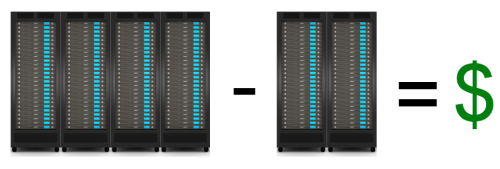
\includegraphics[scale = 0.6]{images/1}
	\end{center}
	\end{figure}

    \vspace*{-0.6cm}
	\hrule \hrule \hrule
	\vspace{0.5cm}
	\textsc{\Large CS 490 :RnD Project}\\[0.5cm]
	% Title
	{\huge \bfseries Dynamic Server Consolidation Problem (DSCP)} \\[0.5cm]
	\hrule \hrule \hrule
	\vspace{4cm}

	% Author and supervisor
	\begin{minipage}{0.5\textwidth}
	\begin{flushleft} \large
		\emph{By:} \\
		Aman Mangal (100050015) \\
		Amit Panghal (100050016)
	\end{flushleft}
	\end{minipage}
	\begin{minipage}{0.4\textwidth}
	\begin{flushright} \large
		\emph{Coordinator:} \\
		Prof. Varsha Apte
	\end{flushright}
	\end{minipage}
	\vspace{1cm}

	% Bottom of the page
	{\large \today}
\end{center}
\end{titlepage}
\tableofcontents
\vspace{0.5cm}
\hrule \hrule \hrule
\newpage

\section{Introduction}

\nocite{cormen}
\nocite{coursera}

\bibliographystyle{abbrv}
\bibliography{ref}

\end{document}
